\chapter{\skstitle: synthetic SKS splitting}
\label{chapter:sks}

Synthetic SKS splitting is computed with routines included in FSTRACK (\citet{becker2006epsl}). An additional routine (savstack.f90) is provided to define a grid of seismic stations and, per each seismic station, build a stack of mantle horizontal layers by averaging elastic tensors and densities of crystal aggregates that are located close to the vertical projection of the station at depth and that are loaded from the \texttt{Cijkl*.h5} output file generated with \drexmtitle{} .\\*
\vspace{0.5cm}

\texttt{COMPILE:}\\*

\begin{itemize}
    \item Untar \texttt{fstrack.tar.gz: tar -zxvf fstrack.tar.gz}
    \item Execute the \texttt{Makefile} in \texttt{fstrack/single\_layer}\footnotemark:   \texttt{make}
    \item Execute the \texttt{Makefile} in \texttt{fstrack/multi\_layer}:   \texttt{make}
    \item copy the binary file \texttt{anicake} from \texttt{/fstrack/bin} directory to the \skstitle{} directory containing the bash file \texttt{pbs\_sks}. Directory \texttt{/fstrack} can be now deleted, if wanted.
    \item Execute \texttt{./bash\_compile} in \skstitle{}
\end{itemize}

\footnotetext{Depending on the Intel Fortran Compiler and environment settings, you need to add \texttt{F77=ifort},\texttt{F90=ifort},\texttt{CC=icc} to each of the two \texttt{Makefile}. This is done in the FSTRACK version present in this package}

\vspace{0.5cm}

\texttt{RUN:} submit the \texttt{pbs\_sks} bash file which consecutively runs:\\
\texttt{./stack\_calc args} (generates a stack of horizontal layers with different elastic tensors)\\
\texttt{mpiexec  -np nprocs  ./split\_calc args} (computes splitting paramters averaged over back-azimuth)\\
\\*

\section{Parameter input file(s)}
In \skstitle{}, open the bash file \texttt{pbs\_sks} and set the directory \fonts{cijkl\_dir} (String) where the \cijkltitle{} file that you want to process is and its filenumber \fonts{timestep} (4 digit Integer). Other parameters are rarely modified, and thus here not explained (but please feel free to contact the software developer for more infos). The number of processes (nprocs) is defined by the run control parameters (shown as an example in \texttt{pbs\_sks}). 
At first, the code \texttt{stack\_calc}, executed by one process, generate a 2D virtual grid of seismic stations and the underlying vertical stack of homogeneous elastic horizontal layers. Successively SKS splitting is computed by nprocs OpenMPI processes by executing \texttt{split\_calc} (modified after Thorsten Becker).

Set the following parameters in file \texttt{stack\_input.dat} (to be placed in the \fonts{cijkl\_dir} directory) to build the grid of virtual seismic stations (in 2D models, ignore \fonts{nsx3, i3first, i3last}):

\begin{itemize}
    \item \fonts{nsx1}: Integer. Number of seismic stations along horizontal axis 1 of the domain defined below
    \item \fonts{nsx3}: Integer. Number of seismic stations along horizontal axis 3 of the domain defined below
    \item \fonts{depthaxis}: Integer
    \begin{itemize}
	    \item[] \fonts{0}: vertical axis positive downward
        \item[] \fonts{1}: vertical axis positive upward
    \end{itemize}
\end{itemize}
    
Define the domain where to set the grid of seismic stations, and the volume enclosing the Lagrangian crystal aggregates sampled by the SKS waves. As SKS waves are mostly sensitive to anisotropy at upper mantle depths (\citet{sieminski2008bssa}), the vertical extent of the domain is usually that of the upper mantle.
\begin{itemize}
    \item \fonts{i1first}, \fonts{i1last}: seismic stations grid and Lagrangian domain axis 1: min, max coordinates (in unit length in cartesian coord.; in degrees in polar/spherical coord.).  
    \item \fonts{i2first}, \fonts{i2last}: Lagrangian domain axis 2: min, max coordinates (in unit length).  
    \item \fonts{i3first}, \fonts{i3last}: seismic stations grid and Lagrangian domain axis 3: min, max coordinates (in unit length in cartesian coord.; in degrees in spherical coord.).
    \item \fonts{maxdist}: maximum horizontal distance of mantle aggregates to be used for the interpolation of density and elastic tensor from the vertical projection at depth of the seismic station (in unit length). As the Fresnel zone of SKS waves is 100-200 km in the upper mantle, maxdist is tipically set to 50-100 km.
    \item \fonts{minlayer}: minimum thickness of each mantle layer (in unit length). This is to avoid a very slow computation resulting from the formation of too many horizontal mantle layers when Lagrangian aggregates are densely packed. The max. number of layers set in anicake.F is 500. 
    \item \fonts{Xscale}: scaling factor used to convert depth in km as Depth [km] = Depth [geodynamic model units] $\cdot$ \fonts{Xscale}. As an example, if depth is defined in meters in the geodynamic model, \fonts{Xscale} must be set equal to $10^{-3}$.  
\end{itemize}

\section{Compute SKS splitting}
By running \texttt{./calc\_split}, the seismic stations position and vertical stack of averaged elastic tensors scaled by density are saved in directory \fonts{cijkl\_dir}\texttt{/seismic\_stations}, while the apparent SKS splitting computed as a function of the back-azimuth every 5 degrees are saved in files \fonts{cijkl\_dir}\texttt{/splitting/split$*$.dat.gz}, where $*$ is the seismic station number. \\*
The azimuthally averaged fast azimuth and delay times, together with standard deviations and station position, are saved in \fonts{cijkl\_dir}\texttt{/splitting/split.0.$*$.staat}, where $*$ is the \cijkltitle{} file number.\\*

\section{SKS splitting visualization}
Files \texttt{split.0.$*$.staat} can be processed with file \texttt{/viz/read\_sks\_splitting.m}, by setting the input parameters. The script plots the SKS splitting averages for a quick view, and generates \texttt{$*$.xmf} and \texttt{$*$.h5} files for visualization in Paraview via the Glyph plot filter. In this way, the SKS data can be superimposed over the geodynamic model and/or the Eulerian grids generated with \viztomotitle{}   (Fig. \ref{fig:radial+sks}). 

Examples of \texttt{stack\_input.dat} and \texttt{read\_sks\_splitting.m} are available for each of the models shown the cookbooks chapter \ref{chapter:cookbooks}.

\begin{figure}
    \centering
    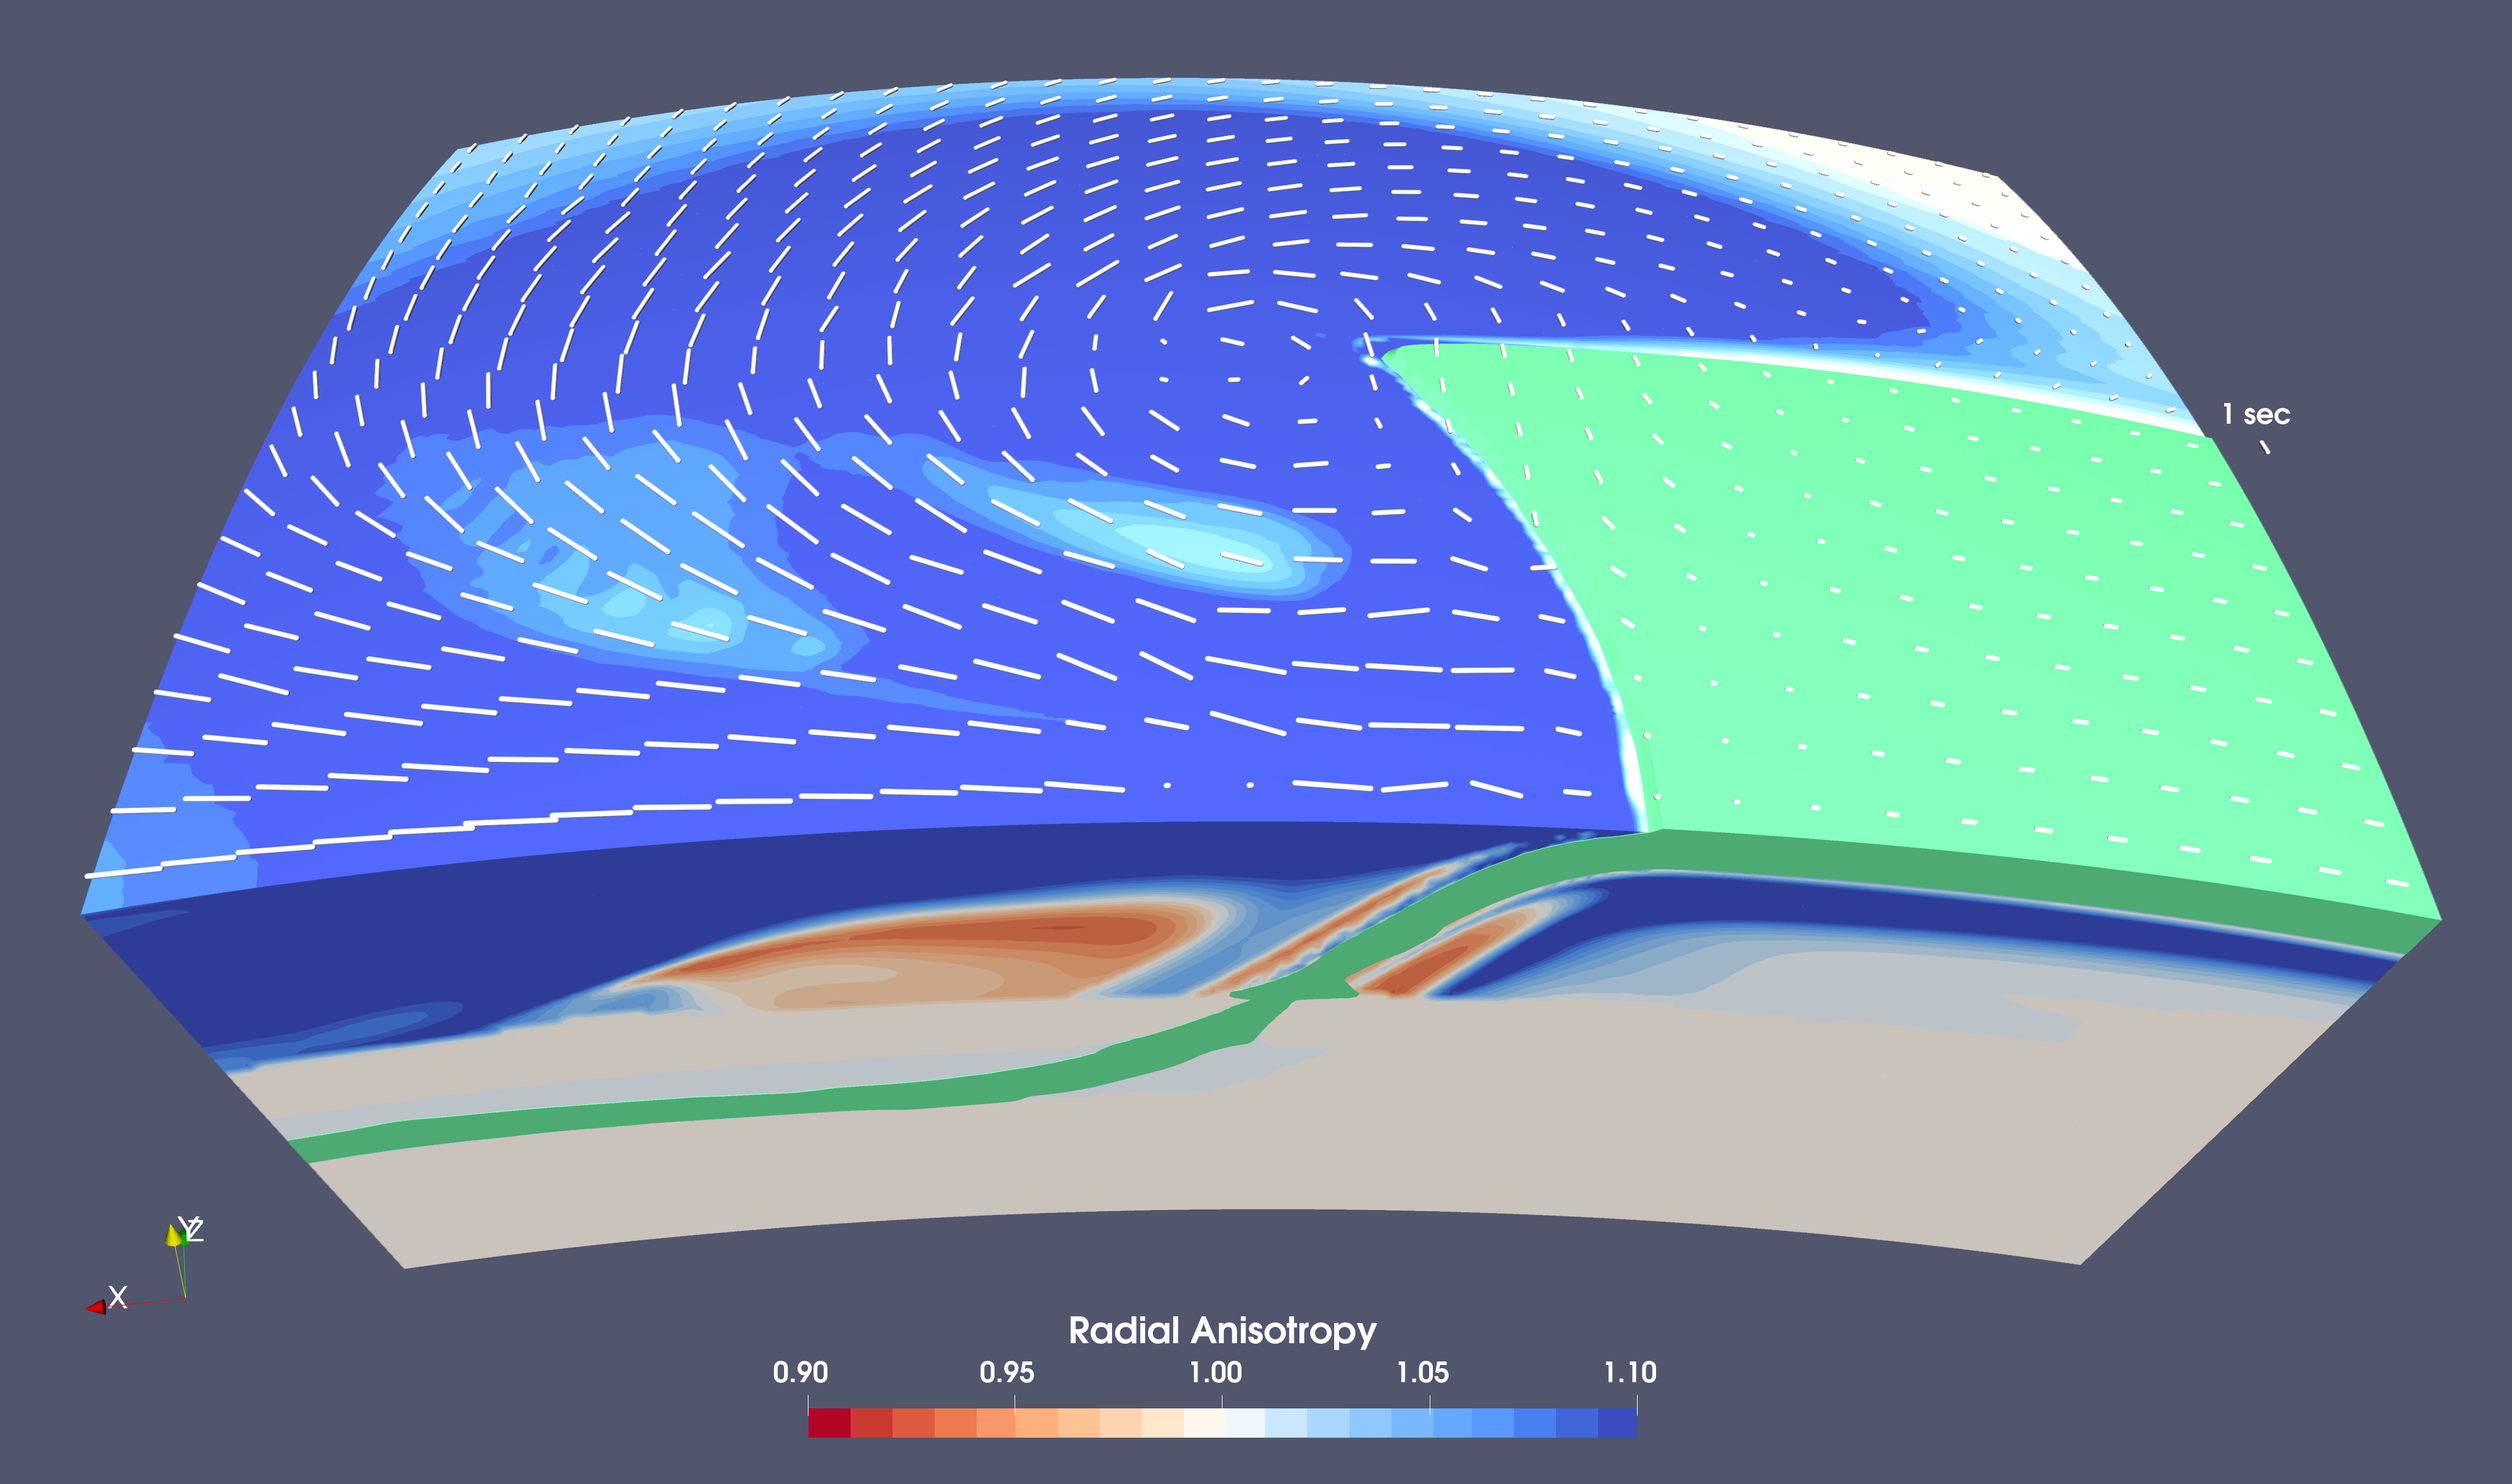
\includegraphics[width=1.0\textwidth]{SKS-SPLIT/Radial+SKS.png}
    \caption{Example of a 3D thermo-mechanical model of subduction in spherical coordinates. The front wall is the subduction zone mid-plane, and it is a symmetric boundary. The green surface enclose material with +1\% Vp anomalies which are related to the cold slab temperatures (note the thicker anomaly around the 410 km discontinuity, which is due to the upwelling of the $Ol \leftrightarrows Wd$ phase transition). The volume is color coded according to radial anisotropy and it has been generated with \viztomotitle{} after running \drexmtitle. The white bars are the mean SKS splitting for each of the seismic stations computed with the \skstitle{} software.}
    \label{fig:radial+sks}
\end{figure}




  



 
